\documentclass[11pt,twocolumn,oneside,openany,headings=optiontotoc,11pt,numbers=noenddot]{article}

\usepackage[a4paper]{geometry}
\usepackage[utf8]{inputenc}
\usepackage[T1]{fontenc}
\usepackage{lmodern}
\usepackage[ngerman]{babel}
\usepackage{ngerman}

\usepackage[onehalfspacing]{setspace}

\usepackage{fancyhdr}
\usepackage{fancybox}

\usepackage{rotating}
\usepackage{varwidth}

%Struktogramme
\usepackage[german,curves]{struktex}

\usepackage{pdflscape}
\usepackage{changepage}
\usepackage{graphicx}
\usepackage[bottom]{footmisc}
\usepackage{transparent}
\usepackage{graphbox}
\graphicspath{
	{Pics/PDFs/}
	{Pics/JPGs/}
	{Pics/PNGs/}
}
\usepackage{caption}
\usepackage{wrapfig}
\usepackage{marginnote}
\usepackage{tabularx}
\usepackage{dashrule}
\usepackage{soulutf8}
\usepackage{hhline}
%arydshln suppresses vertical lines in table
%\usepackage{arydshln}
\usepackage{multirow}
\usepackage{enumerate}
\usepackage[hidelinks]{hyperref}
\usepackage{listings}

\usepackage[table]{xcolor}
\usepackage{array}
\usepackage{enumitem,amssymb,amsmath}
\usepackage{interval}
\usepackage{cancel}
\usepackage{stmaryrd}
\usepackage{wasysym}
\usepackage{polynom}
\usepackage{diagbox}
\usepackage{dashrule}
\usepackage{framed}
\usepackage{mdframed}
\usepackage{karnaugh-map}
\usepackage{pdfpages}

\usepackage{blindtext}

\usepackage{eso-pic}

\usepackage{amssymb}
\usepackage{eurosym}

\usepackage[pages=some]{background}
\pagestyle{headings}
\renewcommand{\headrulewidth}{0.2pt}
\renewcommand{\footrulewidth}{0.2pt}
\newcommand*{\underdownarrow}[2]{\ensuremath{\underset{\overset{\Big\downarrow}{#2}}{#1}}}
\setlength{\fboxsep}{5pt}
\newcommand{\explainBelow}[3]{\underbrace{#1}_{\parbox{\widthof{#3}}{\footnotesize\raggedright #2}}}
\newcommand{\explainAbove}[3]{\overbrace{#1}^{\parbox{\widthof{#3}}{\footnotesize\raggedright #2}}}
\newcommand\footnoteref[1]{\protected@xdef\@thefnmark{\ref{#1}}\@footnotemark}


% Codestyle defined
\definecolor{codegreen}{rgb}{0,0.6,0}
\definecolor{codegray}{rgb}{0.5,0.5,0.5}
\definecolor{codepurple}{rgb}{0.58,0,0.82}
\definecolor{backcolour}{rgb}{0.95,0.95,0.92}
\definecolor{deepgreen}{rgb}{0,0.5,0}
\definecolor{darkblue}{rgb}{0,0,0.65}
\definecolor{mauve}{rgb}{0.40, 0.19,0.28}
\colorlet{exceptioncolour}{yellow!50!red}
\colorlet{commandcolour}{blue!60!black}
\colorlet{numpycolour}{blue!60!green}
\colorlet{specmethodcolour}{violet}

%Neue Spaltendefinition
\newcolumntype{L}[1]{>{\raggedright\let\newline\\\arraybackslash\hspace{0pt}}m{#1}}
\newcolumntype{M}{>{\centering\arraybackslash}X}
\newcommand{\cmnt}[1]{\ignorespaces}
%Textausrichtung ändern
\newcommand\tabrotate[1]{\rotatebox{90}{\raggedright#1\hspace{\tabcolsep}}}

%Intervall-Konfig
\intervalconfig {
	soft open fences
}

%Bash
\lstdefinestyle{BashInputStyle}{
	language=bash,
	basicstyle=\small\sffamily,
	backgroundcolor=\color{backcolour},
	columns=fullflexible,
	backgroundcolor=\color{backcolour},
	breaklines=true,
}
%Java
\lstdefinestyle{JavaInputStyle}{
	language=Java,
	backgroundcolor=\color{backcolour},
	aboveskip=1mm,
	belowskip=1mm,
	showstringspaces=false,
	columns=flexible,
	basicstyle={\footnotesize\ttfamily},
	numberstyle={\tiny},
	numbers=none,
	keywordstyle=\color{purple},,
	commentstyle=\color{deepgreen},
	stringstyle=\color{blue},
	emph={out},
	emphstyle=\color{darkblue},
	emph={[2]rand},
	emphstyle=[2]\color{specmethodcolour},
	breaklines=true,
	breakatwhitespace=true,
	tabsize=2,
}
%Python
\lstdefinestyle{PythonInputStyle}{
	language=Python,
	alsoletter={1234567890},
	aboveskip=1ex,
	basicstyle=\footnotesize,
	breaklines=true,
	breakatwhitespace= true,
	backgroundcolor=\color{backcolour},
	commentstyle=\color{red},
	otherkeywords={\ , \}, \{, \&,\|},
	emph={and,break,class,continue,def,yield,del,elif,else,%
		except,exec,finally,for,from,global,if,import,in,%
		lambda,not,or,pass,print,raise,return,try,while,assert},
	emphstyle=\color{exceptioncolour},
	emph={[2]True,False,None,min},
	emphstyle=[2]\color{specmethodcolour},
	emph={[3]object,type,isinstance,copy,deepcopy,zip,enumerate,reversed,list,len,dict,tuple,xrange,append,execfile,real,imag,reduce,str,repr},
	emphstyle=[3]\color{commandcolour},
	emph={[4]ode, fsolve, sqrt, exp, sin, cos, arccos, pi,  array, norm, solve, dot, arange, , isscalar, max, sum, flatten, shape, reshape, find, any, all, abs, plot, linspace, legend, quad, polyval,polyfit, hstack, concatenate,vstack,column_stack,empty,zeros,ones,rand,vander,grid,pcolor,eig,eigs,eigvals,svd,qr,tan,det,logspace,roll,mean,cumsum,cumprod,diff,vectorize,lstsq,cla,eye,xlabel,ylabel,squeeze},
	emphstyle=[4]\color{numpycolour},
	emph={[5]__init__,__add__,__mul__,__div__,__sub__,__call__,__getitem__,__setitem__,__eq__,__ne__,__nonzero__,__rmul__,__radd__,__repr__,__str__,__get__,__truediv__,__pow__,__name__,__future__,__all__},
	emphstyle=[5]\color{specmethodcolour},
	emph={[6]assert,range,yield},
	emphstyle=[6]\color{specmethodcolour}\bfseries,
	emph={[7]Exception,NameError,IndexError,SyntaxError,TypeError,ValueError,OverflowError,ZeroDivisionError,KeyboardInterrupt},
	emphstyle=[7]\color{specmethodcolour}\bfseries,
	emph={[8]taster,send,sendMail,capture,check,noMsg,go,move,switch,humTem,ventilate,buzz},
	emphstyle=[8]\color{blue},
	keywordstyle=\color{blue}\bfseries,
	rulecolor=\color{black!40},
	showstringspaces=false,
	stringstyle=\color{deepgreen}
}

\lstset{literate=%
	{Ö}{{\"O}}1
	{Ä}{{\"A}}1
	{Ü}{{\"U}}1
	{ß}{{\ss}}1
	{ü}{{\"u}}1
	{ä}{{\"a}}1
	{ö}{{\"o}}1
}

% Neue Klassenarbeits-Umgebung
\newenvironment{worksheet}[3]
% Begin-Bereich
{
	\newpage
	\sffamily
	\setcounter{page}{1}
	\ClearShipoutPicture
	\AddToShipoutPicture{
		\put(55,761){{
				\mbox{\parbox{385\unitlength}{\tiny \color{codegray}BBS I Mainz, #1 \newline #2
						\newline #3
					}
				}
			}
		}
		\put(455,761){{
				\mbox{\hspace{0.3cm}
\includegraphics[width=0.2\textwidth]{../../logo.pdf}}
			}
		}
	}
}
% End-Bereich
{
	\clearpage
	\ClearShipoutPicture
}

\setlength{\columnsep}{3em}
\setlength{\columnseprule}{0.5pt}

\geometry{left=2.00cm,right=2.00cm,top=3.00cm,bottom=1.00cm,includeheadfoot}
\pagenumbering{gobble}
\pagestyle{empty}

\begin{document}
	\begin{worksheet}{BS FI 16}{2. Lehrjahr, LF 9 - Öffentliche Netze}{Informationen zu \glqq{}Strukturierte Verkabelung\grqq{}}
		\section{Strukturierte Verkabelung}
		Strukturierte Verkabelung ist die Verkabelung eines Gebäudes oder einer Reihe von Gebäuden mit Kabeln, Anschlussdosen, Etagenverteilern, Gebäudeverteilern und Standortverteilern. Ziel ist, die Anforderungen aller potenziellen Nutzer des Gebäudes während seiner gesamten Lebensdauer zu erfüllen, ohne erneut verkabeln zu müssen.\\
		\par\noindent
		Mit diesem Verfahren der Vorverkabelung der Gebäudeinfrastruktur ist es möglich, ein universelles für den Benutzer vollständig durchschaubares System zu installieren - ein universelles, anwendungsunabhängiges Netz.\\
		\par\noindent
		Strukturiertes Verkabeln bedeutet, dass das System hierarchisch aufgebaut ist. Diese Hierarchie umfasst folgende Ebenen in Bezug auf die Verkabelung:\\
		\par\noindent
		\begin{tabularx}{0.5\textwidth}{X}
			\textbullet \textbf{Primärverkabelung:} zwischen Standort- und Gebäudeverteiler\\
			\textbullet \textbf{Sekundärverkabelung:} zwischen Gebäude- und Etagenverteiler\\
			\textbullet \textbf{Tertiärverkabelung:} zwischen Etagenverteiler und informationstechnischer Anschlussdose\\
			\textbullet \textbf{Arbeitsplatzverkabelung:} zwischen Anschlussdose und Endgerät
		\end{tabularx}\\
		\par\noindent
		Hierarchie der Strukturierten Verkabelung:\\
		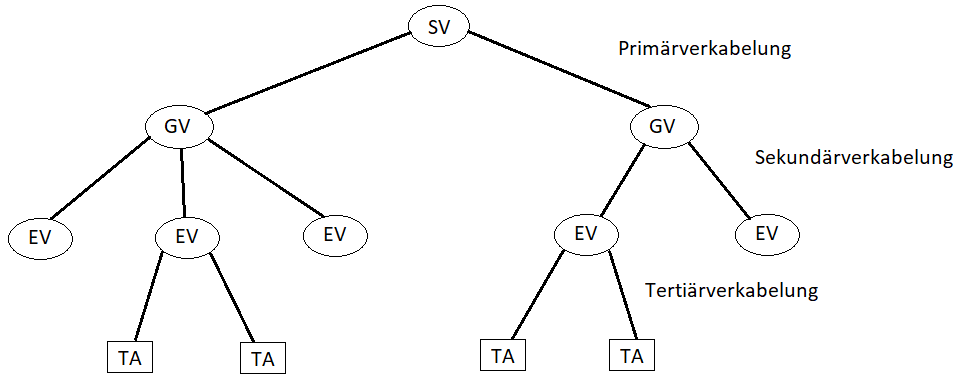
\includegraphics[scale=0.45]{Bilder/struktVerk.png}\\
		\tiny{SV = Standortverteiler; GV = Gebäudeverteiler; EV = Etagenverteiler; TA = informationstechnische Anschlussdose}\\
		\normalsize
		\newpage\noindent
		Umsetzung der strukturierten Verkabelung in die Standort- und Gebäudeverkabelung:\\
		\begin{center}
			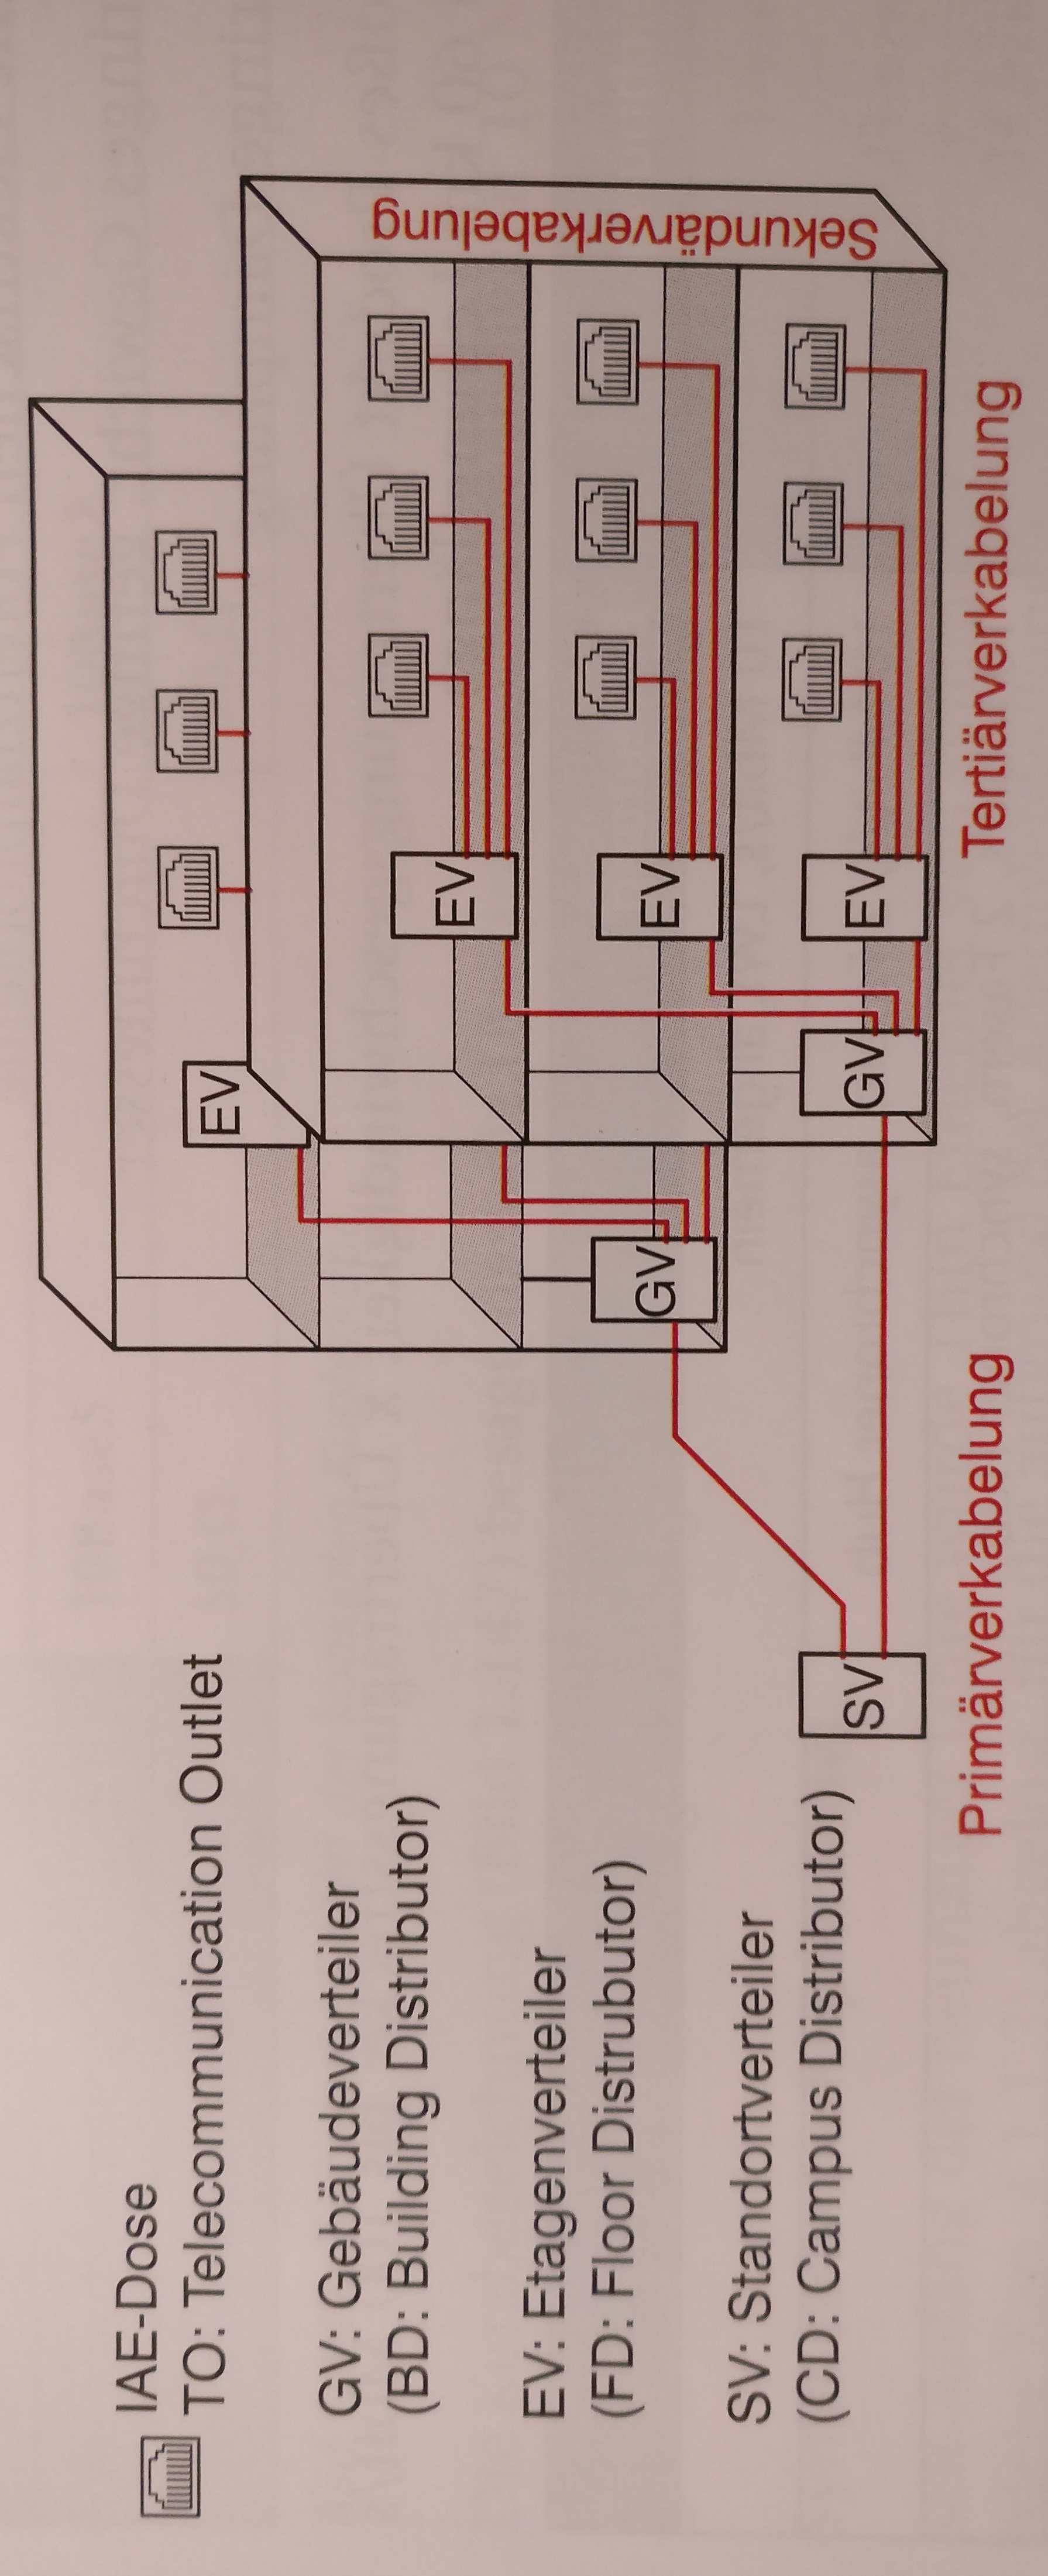
\includegraphics[scale=0.1]{Bilder/Verkabelungsbereiche.jpg}
		\end{center}
		\newpage\noindent
		\subsection*{Verkabelungsstruktur} Der Standard EIA/TIA 568 (comercial building wiring standard) geht von einer strukturierten Verkabelung aus, die zwischen unterschiedlichen Verkabelungsstufen unterscheidet. Gebäude werden untereinander durch die sogenannte Geländeverkabelung (Primärbereich) verbunden. Innerhalb des Gebäudes gibt es Etagen. Die Etagen werden untereinander durch die sogenannte Verkabelung im Steigbereich (Sekundärbereich) verbunden.\\
		Innerhalb der Etagen gibt es Technikräume, die die gesamten Komponenten der strukturierten Verkabelung enthalten müssen und darüber hinaus für den LAN-Betrieb wichtige Geräte wie Hubs, Bridges, Switches, Router oder Server enthalten können. Untereinander sind die Technikräume üblicherweise mit der Steigbereichtechnk verbunden. Im Etagenbereich (Tertiärberich) werden die Endgeräteanschlüsse von den Technikräumen aus versorgt. Je nach Verkabelungssystem differieren die Konzepte, die benutzen Übertragungsmedien, die Verteil- und die Anschlusstechnik.\\
		\subsection*{Primärverkabelung, Geländeverkabelung} Die Geländeverkabelung integriert die in den einzelnen Gebäuden bestehenden Subnetze. An die Geländeverkabelung werden folgende Anforderungen gestellt:\\
		Überbrückung großer Entfernung, Blitzschutz, Einstreusicherheit, Ausfallsicherheit, hohe Verfügbarkeit, Wartbarkeit, Potenzialtrennung zwischen Gebäudeerdung, hohe Übertragungskapazität.\\
		\par\noindent
		All dies kann z.B. im Rahmen einer gut gut durchdachten Glasfaserverkabelung erreicht werden, da die Glasfaser gerade mit den genannten Anforderungen keinerlei Probleme hat und bei anderen Kabeltypen hierfür besondere Maßnahmen erforderlich werden können.
		\subsection*{Gebäudeverkabelung} Die Gebäudeverkabelung integriert die Etagennetze und die Etagenverkabelung und bindet die einzelnen räumlichen Einheiten an das Netz. Von der Gebäudeverkabelung wird gefordert:\\
		Modularität bei der Verkabelung der Etagen oder Bereiche, Aufbau und Betrieb von begehbaren Gebäude- und Etagenverteilern, wartbares Kabelsystem zur schnellen Fehlersuche, netzwerkunabhängige Verkabelung und Anpassbarkeit an die vorhandenen Steigbereiche.
		\subsection*{Etagenverkabelung} An die Etagenverkabelung(Tertiärbereich) werden folgende Anforderungen gestellt:\\
		Anbindung von Wanddosen in den Büros oder Arbeitsbereichen an den Etagenverteiler; universelle Dosen- und Steckertechnik, gegebenenfalls aufgeteilt nach Sprach- und Datenübertragung; Nutzung geeigneter Kabelwegsysteme, wie Doppelbodenkanäle, abgehängte Decken, begehbare Kabelkanäle; netzunabhängige Verkabelung; beliebige Versetzbarkeit on Arbeitsplätzen; Erweiterbarkeit; Flexibilität.
		\newpage\noindent
		\begin{center}
			\includegraphics[scale=1.3]{Bilder/Kabellaenge1.png}
		\end{center}
		\newpage\noindent
		\subsection*{Zulässige Kabellängen}
		\begin{center}
			\includegraphics[scale=1.3]{Bilder/Kabellaenge2.png}
		\end{center}
		ASG = anwendungsspezifisches Gerät\\
		Die Gesamtlänge \(A + B + C\) darf 100m nicht überschteigen.\\
	\end{worksheet}
\end{document}